\documentclass[11pt,letterpaper]{article}

\usepackage[utf8]{inputenc}
%%% PACKAGES
\usepackage{array}
\usepackage{verbatim}
\usepackage{subfig}
\usepackage[margin=1in]{geometry}
\usepackage{graphicx}

\usepackage{hyperref}
\usepackage{hypcap}

\title{Business Organization}
\author{PICA, LLC.}
%\date{} % Activate to display a given date or no date (if empty),
         % otherwise the current date is printed 

\begin{document}
\maketitle

\section{Plan of Operation}


\subsection{Legal form of ownership}
The business shall be formed as a limited liability company under the name "PICA, LLC."

\subsection{Company structure}

\begin{figure}[htbp]
 \begin{center}
  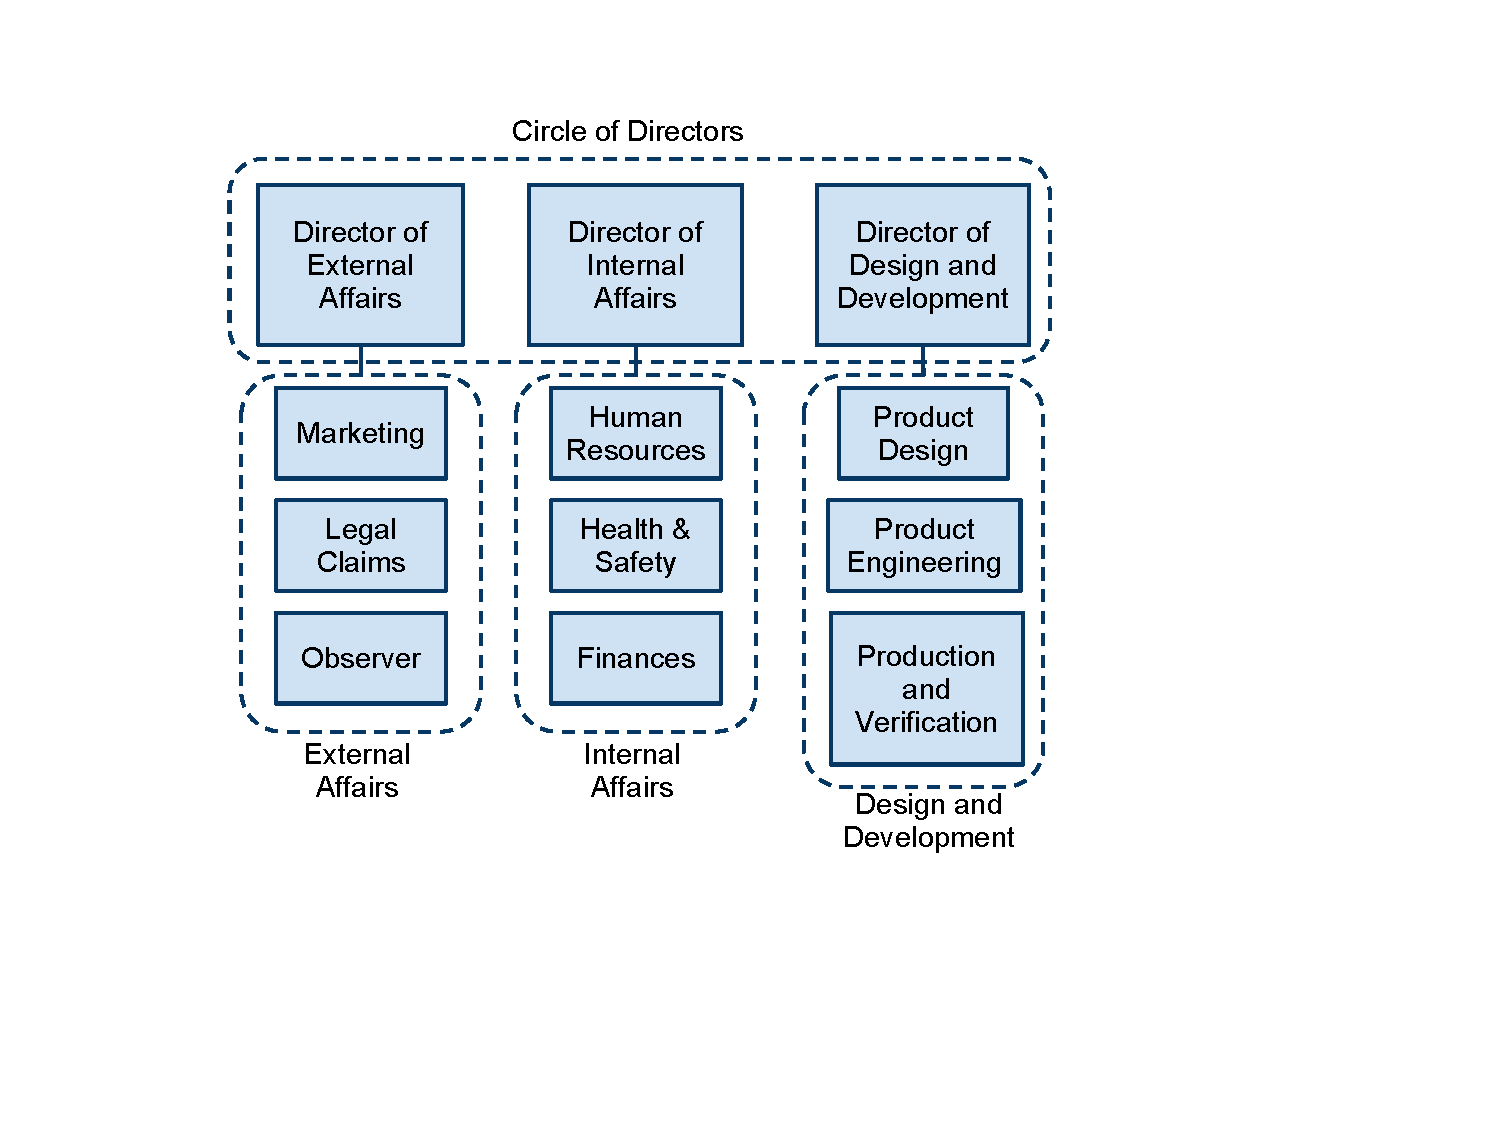
\includegraphics[trim=1.5in 1.75in 3in 0.75in,clip,width=0.6\textwidth]{includes/PICA_LLC_Org_Chart}
 \end{center}
 \caption{Proposed Organization Chart for PICA, LLC.}
 \label{fig:org-chart}
\end{figure}

\subsubsection{Select explanations of Figure \ref{fig:org-chart} }
The Internal Affairs directorate shall provide certain services to the other directorates and departmetns. For example, Internal Affairs includes the Human Resources division, but the other directorates will of course require the services of the HR division in order to hire new employees. Similarly, the finances division will provide budgeting information to the other divisions and directorates.

The other two directorates do not provide services to the other directorates. The one exception to this is the Observer function of the External Affairs directorate: its purpose is to monitor the business and legal climate in terms to demands and regulations, then inform the appropriate divisions. This could be spun off into its own directorate, but will likely not employ enough people to grant it a director and a direct voice in the Circle of Directors.

\subsection{Decision-making authority chain}
The final authority on a decision shall be vested in the Circle of Directors, but their authority shall not be required in every decision. The Circle of Directors shall have the exclusive power to make decisions regarding the direction of the business and the relationships between the directorates. Other issues may rise to the Circle if they cannot be resolved at a lower level or if the scope of the decision cannot be contained to one directorate. Otherwise, decisions that are limited in scope to any particular group or body shall be resolved within that body with the advice of the applicable Internal Affairs departments.



\subsection{Compensation/benefits package}
All employees shall be compensated fairly and in proportion to the scope of their decisions and actions. The company shall provide benefits packages including medical- prescription, vision, and dental plans. In addition, the company shall also provide a cafeteria and snacks for its employees to enjoy within moderation. The lowest Engineering position shall pay an annual salary of \$55,000, with up to 50\% increases in pay for each level of management ascended. Employees in other directorates will earn an annual salary of \$35,000, with a similar reward for ascending management. Employees shall receive raises in pay for distinguishing their work from that of their peers.


\end{document}
